\title[JASA/draft]{Under-ice acoustic navigation using real-time model-aided range estimation}
\author{EeShan C. Bhatt}
\email{ebhatt@whoi.edu}
\affiliation{MIT-WHOI Joint Program in Oceanography/Applied Ocean Science \& Engineering, Cambridge and Woods Hole, MA, USA}
\affiliation{Department of Mechanical Engineering, Massachusetts Institute of Technology, Cambridge, MA}
\author{Oscar Viquez}
\affiliation{Department of Mechanical Engineering, Massachusetts Institute of Technology, Cambridge, MA}
\author{Henrik Schmidt}
\email{henrik@mit.edu}
\affiliation{Department of Mechanical Engineering, Massachusetts Institute of Technology, Cambridge, MA}

% \author{Author Four}
% \email{author.four@university.edu}
% \affiliation{Department2,  University2, City, State ZipCode, Country}

\preprint{Bhatt, JASA}   %  if you want want this message to appear in upper right corner of title page

\date{\today}

% The motivation behind this work is to improve the standard LBL navigation’s conversion of travel time to range for an under-ice environment in a way that could be generalized to any acoustic waveguide. To do this, we introduce the Minimal Bounce Criteria method to operationalize real-time acoustic modeling into an effective horizontal group velocity estimate.

% 	This system was implemented on an autonomous underwater vehicle (AUV) on multiple missions, including an 11 km untethered, under-ice deployment, in March 2020. The AUV was deployed through a hydrohole from Topside and due to a disk error, stalled underneath the ice surface while transmitting its perceived location. The AUV was found within a meter away from its reported location, which serves as strong (but qualitative) evidence of the navigation performance provided by the single group velocity calculation. Because the navigation updates throughout the AUV mission have no GPS ground truth to compare to, this paper evaluates the same system performance across the GPS-navigated LBL beacons. 

% 	The real-time error from the Nearest Bounce Criteria (NBC) achieves a mean absolute positioning error of 11 m. Upon further evaluation of the acoustic events, the Minimal Bounce Criteria (MBC) is run in the same automated pipeline in post-processing (akin to real-time computational constraints and needs) and achieves an error of roughly 3 m.

% 	Both the NBC and MBC pseudorange estimations are compared to the GPS data on the LBL beacons. The error itself is small and the pattern of error exhibited indicates that the GPS ground truth data has significant noise (drift) that is not replicated by either pseudorange estimation method. For the MBC in particular, the post-processing error is within the precision of the GPS sensor, suggesting that its performance rivals that of GPS.

\begin{abstract}
The long baseline (LBL) underwater navigation paradigm relies on the conversion of recorded travel time to range to trilaterate for position.
For real-time operations, this conversion has assumed an isovelocity sound speed.
For re-navigation in post-processing, computationally and/or labor intensive acoustic modeling may be employed to reduce uncertainty driven by multipath arrivals.
This work demonstrates a real-time ray-based prediction method of the effective sound speed along a path from source to receiver to minimize vehicle position error.
\llabel{2.1} This method was implemented for a small scale AUV-LBL system in March 2020, in the Beaufort Sea, in total ice-covered conditions and a double ducted acoustic propagation environment.
The vehicle was successfully deployed and recovered.
\llabel{2.2} Given the lack of GPS data throughout the vehicle's mission, however, the pseudorange performance is first evaluated on connections between GPS-linked beacons.
The real-time ranging error between beacons is roughly 11 meters at distances up to 3 km.
But a consistent overestimation in the real-time method, the Minimum Bounce Criteria (MBC), provides insights for improved eigenray filtering, which we call the Nearest Bounce Criteria (NBC).
An operationally equivalent pipeline is used to re-position the LBL beacons and re-navigate the AUV, using a modeled, historical, and a locally observed sound speed profile.
The median re-positioning errors for the MBC and NBC are roughly 10 and 3 meters, respectively.
The improved trilateration performance for re-positioning and re-navigation suggests that this approach effectively extends the single meter accuracy of the deployed GNSS units into the water column.

\end{abstract}

%% pacs numbers not used

\maketitle

% =========================================================================== %
% =========================================================================== %

\section{Introduction}
\label{sec:1}  
Autonomous underwater vehicles (AUVs) are increasingly capable platforms to explore and sample the ocean, particularly for remote and/or dangerous regions.
However, navigation uncertainty is a major challenge in considering AUVs as standard tools for oceanographic research.
While land and air-based robots utilize information from Global Navigation Satellite Systems (GNSS) to achieve stunning location accuracy and precision throughout the duration of their missions, AUVs cannot access GNSS while underwater due to the rapid attenuation of electromagnetic waves.
Therefore, underwater vehicles have relied on any combination of dead reckoning, hydrodynamic models, inertial navigation systems, doppler velocity logs, and acoustic baseline positioning systems for navigation \citep{paull_auv_2014}.
Limiting navigation error and drift requires an AUV to periodically stall on the surface and obtain a GNSS fix to reset its position error.
This foolproof method of self-positioning is undesirable for stealth, adverse weather conditions, and mission efficiency, and inaccessible in a GNSS-denied situation like an ice-covered environment.

% introduce LBL and precise statement of work
Of underwater acoustic navigation systems, long baseline (LBL) is the most GPS-like in style and scale, and most appropriate for mitigating drift without overburdening computation or payload size on the vehicle \citep{paull_auv_2014,van_uffelen_global_2021}.
The state-of-the-art for LBL outsources depth to a pressure sensor and solves the two-dimensional localization problem with an isovelocity, linear scaling between one way travel time (OWTT) and range \citep{eustice_recent_2006,eustice_experimental_2007,webster_preliminary_2009,webster_advances_2012}.
This assumption is valid for short scale operations but oversimplifies propagation for larger and/or complex acoustic environments.
To achieve single meter, GNSS-like performance in a GNSS-denied environment, we demonstrate an embedded ray-based data processing algorithm to convert recorded OWTTs into pseudorange estimates.
This methodology was integrated onto the AUV Macrura, deployed and recovered in the Beaufort Sea, in March 2020, during the Ice Exercise 2020 (ICEX20).
A physics-driven methodology that received an \textit{in situ} sound speed profile (SSP) was necessary despite the small operational domain because of the relatively high-risk mission environment\textemdash total under-ice conditions and a variable double ducted acoustic environment.

%% rest of the background, JASA style

% PNT
For clarity, we delineate specific definitions for timing, positioning, and navigation from \citep{howe_observing_2019}.
\begin{enumerate}
	\item Timing is the ability to acquire and maintain accurate and precise time anywhere in the domain of interest within user-defined timeliness parameters
	\item Positioning is the ability to accurately and precisely determine one's location referenced to a standard geodetic system
	\item Navigation is the ability to determine current and desired position (relative or absolute) and apply corrections to course, orientation, and speed to attain a desired position anywhere in the domain of concern
\end{enumerate}
Thus, navigation is inherently in real time and depends on positioning; positioning depends on timing.
We also suggest re-navigation and re-positioning as post-processed corollaries, which may include knowledge or processing capabilities not available \textit{in situ}.

% More about LBL navigation
While RAFOS floats championed one way ranging for re-positioning \citep{rossby_rafos_1986,duda_evaluation_2006}, the ability to do so for navigation was facilitated by \llabel{1.11} the advent of the WHOI micro-modem \citep{singh_underwater_2006} and synchronized chip scale atomic clocks \citep{gardner_second_2016}.
AUV navigation efforts have achieved root mean square (RMS) localization error on the order of tens of meters relative to GNSS surface position over less than ten kilometers in shallow \citep{eustice_experimental_2007,kepper_mems_2017,claus_closed-loop_2018} and deep water \citep{,kunz2008deep,jakuba2008long,webster_preliminary_2009}.
However, these efforts all used a nominal sound speed for travel time conversion and the vehicles were limited to shallower isovelocity regimes. 
Localization algorithms that do consider environmental or acoustic uncertainty tend to focus on longer and larger experiments, where spatio-temporal variability cannot be ignored.
These methods have been reserved for post-processing as they can be labor intensive, computationally heavy, and/or require additional information like contemporaneous data.
For example, gliders navigating with kinematic flight models and equipped with acoustic modems were later unambiguously associated with predicted ray arrivals, resulting in roughly a kilometer error and hundred meters uncertainty over basin scale propagation \cite{van_uffelen_estimating_2013}.
A follow up study investigated how a single temporally and spatially averaged SSP could mitigate position error for a four month glider mission \cite{van_uffelen_localization_2016}.
\citet{wu_assessment_2018} cross correlate three days of real acoustic records with synthetic ones generated through ocean model snapshots from HYCOM \cite{chassignet_hycom_2007}.
While potentially applicable for various ocean states, this is reliant on model realism and impractical for real-time operations.
\cite{mikhalevsky_deep_2020} introduces a ``cold start'' algorithm that does not require prior knowledge of track, position, or sound speed information.
The algorithm inputs a four-dimensional ocean model, constrained by tomography data, into a range dependent ray code to isolate the last path detected in a full multipath pattern.
Then, a representative group speed is solved for alongside position in a least squares fashion. 
Their results re-position a floating hydrophone array with an error of 58 m and a standard deviation of 32 m based on six sources 129--450 km away.
This approach remains to be realized for real-time navigation.

Compared to the previous work mentioned, the approach in this paper integrates real-time model-aided data processing to estimate a representative sound speed along a path from source to receiver for small scale navigation, taking advantage of climatology, \textit{in situ} data, and fast acoustic modeling.
An environmentally- and physically-driven relationship between recorded travel time and estimated range is necessary because of the multipath uncertainty brought upon by the increasingly observed double ducted environment in the Beaufort Sea, which some refer to as the ``Beaufort Lens'' \citep{litvak2015acoustics,chen_spectral_2019,chen2020temporal}.

Given that a lens introduces significant ray refraction, the Beaufort Lens is a convenient shorthand for the spatio-temporal variability of the local temperature and sound speed maxima driven by Pacific Summer Water, generally around 50 to 60 m in depth.
From top to bottom, there is less saline surface water via ice melt; warm saline Pacific Summer Water; cold Pacific Winter Water; warm saline Atlantic water, and then Arctic Deep Water \citep{duda_acoustic_2017,ballard_temporal_2020}.
With this intense stratification, the lens creates a unique double ducted environment that has drastic consequences for acoustic communication and navigation compared to historically observed monotonically increasing sound speed profile \citep{schmidt2016acoustic}.
Transmissions in the upper duct, between the surface ice and the lens, experience minimal attenuation but degrade in signal coherence with repeated reflections under the ice.
In lower duct, between the lens and its conjugate depth in the Atlantic water, sound above 350 Hz is trapped effectively for long range propagation \citep{poulsen2016acoustic}.

Thorough reviews of uncrewed vehicle operations in polar environments can be found in \citep{norgren_unmanned_2014} and \citep{barker_scientific_2020}; there is no comparable work in the Arctic for a short range AUV deployment in the Beaufort Lens.
Seminal \citep{brooke1981arcs,jackson1983autonomous,light1989autonomous,bellingham1995auv,hayes2002determining} and more recent AUV deployments \citep{jakuba2008long,kunz_deep_2008,kukulya2010under,plueddemann_autonomous_2012,timmermans2013scales,fossum2021adaptive} witnessed the classical upward refracting sound speed profile that is amenable to an isovelocity assumption.

Of note, despite different platforms and scales, are recent glider deployments in the Canada Basin.
In 2014, in partially ice-covered conditions, a long range LBL system with WHOI micro-modems at 100 m exploited the lower duct for long range communication with two gliders \citep{freitag_long_2015,webster2015towards}.
The sound speed value measured at the time of reception was used to estimate range in post-processing.
The beacon-to-beacon performance was excellent, achieving contact at ranges greater than 200 km with a position uncertainty of 40 m.
The beacon-to-glider performance, however, deteriorated due to missed contacts outside the duct.
In 2017, gliders were deployed in a region with no ice coverage. 
Ranges were linearly scaled by a statistical description of sound speed observations taken during the experiment, 1450 $\pm$ 6.5 m/s \citep{graupe2019preliminary}.
This resulted in an error of 550 m, which was reduced by a factor between 4 and 5, depending on the dive, using a post-processing acoustic arrival matching method.
Both cases exploit the lower duct for high fidelity communication at long ranges.
Unintuitively, the smaller nature of our deployment during ICEX20 is not a simplifying factor.
For source depths typical to vehicle operations, 30 to 200 m, a shadow zone spans from 2 to 6 kilometers in range \citep{schmidt2016acoustic}.

The paper is organized as follows. Section \ref{sec:icex20} details the experimental conditions during ICEX20.
Given that there is no GNSS ground truth for the vehicle position while underway, we first evaluate the real-time ranging performance of GPS-linked beacon-to-beacon communication events in section \ref{sec:realtime}.
Section \ref{sec:post} uses insights from field data to introduce a new ray filtering algorithm to improve range estimation.
Section \ref{sec:trilat} emulates the real-time processing pipeline to re-position beacon-to-beacon events and re-navigate AUV Macrura.

\clearpage
\section{ICEX20 conditions and experiment design}\label{sec:icex20}

\begin{figure}[h!]
	\centering
	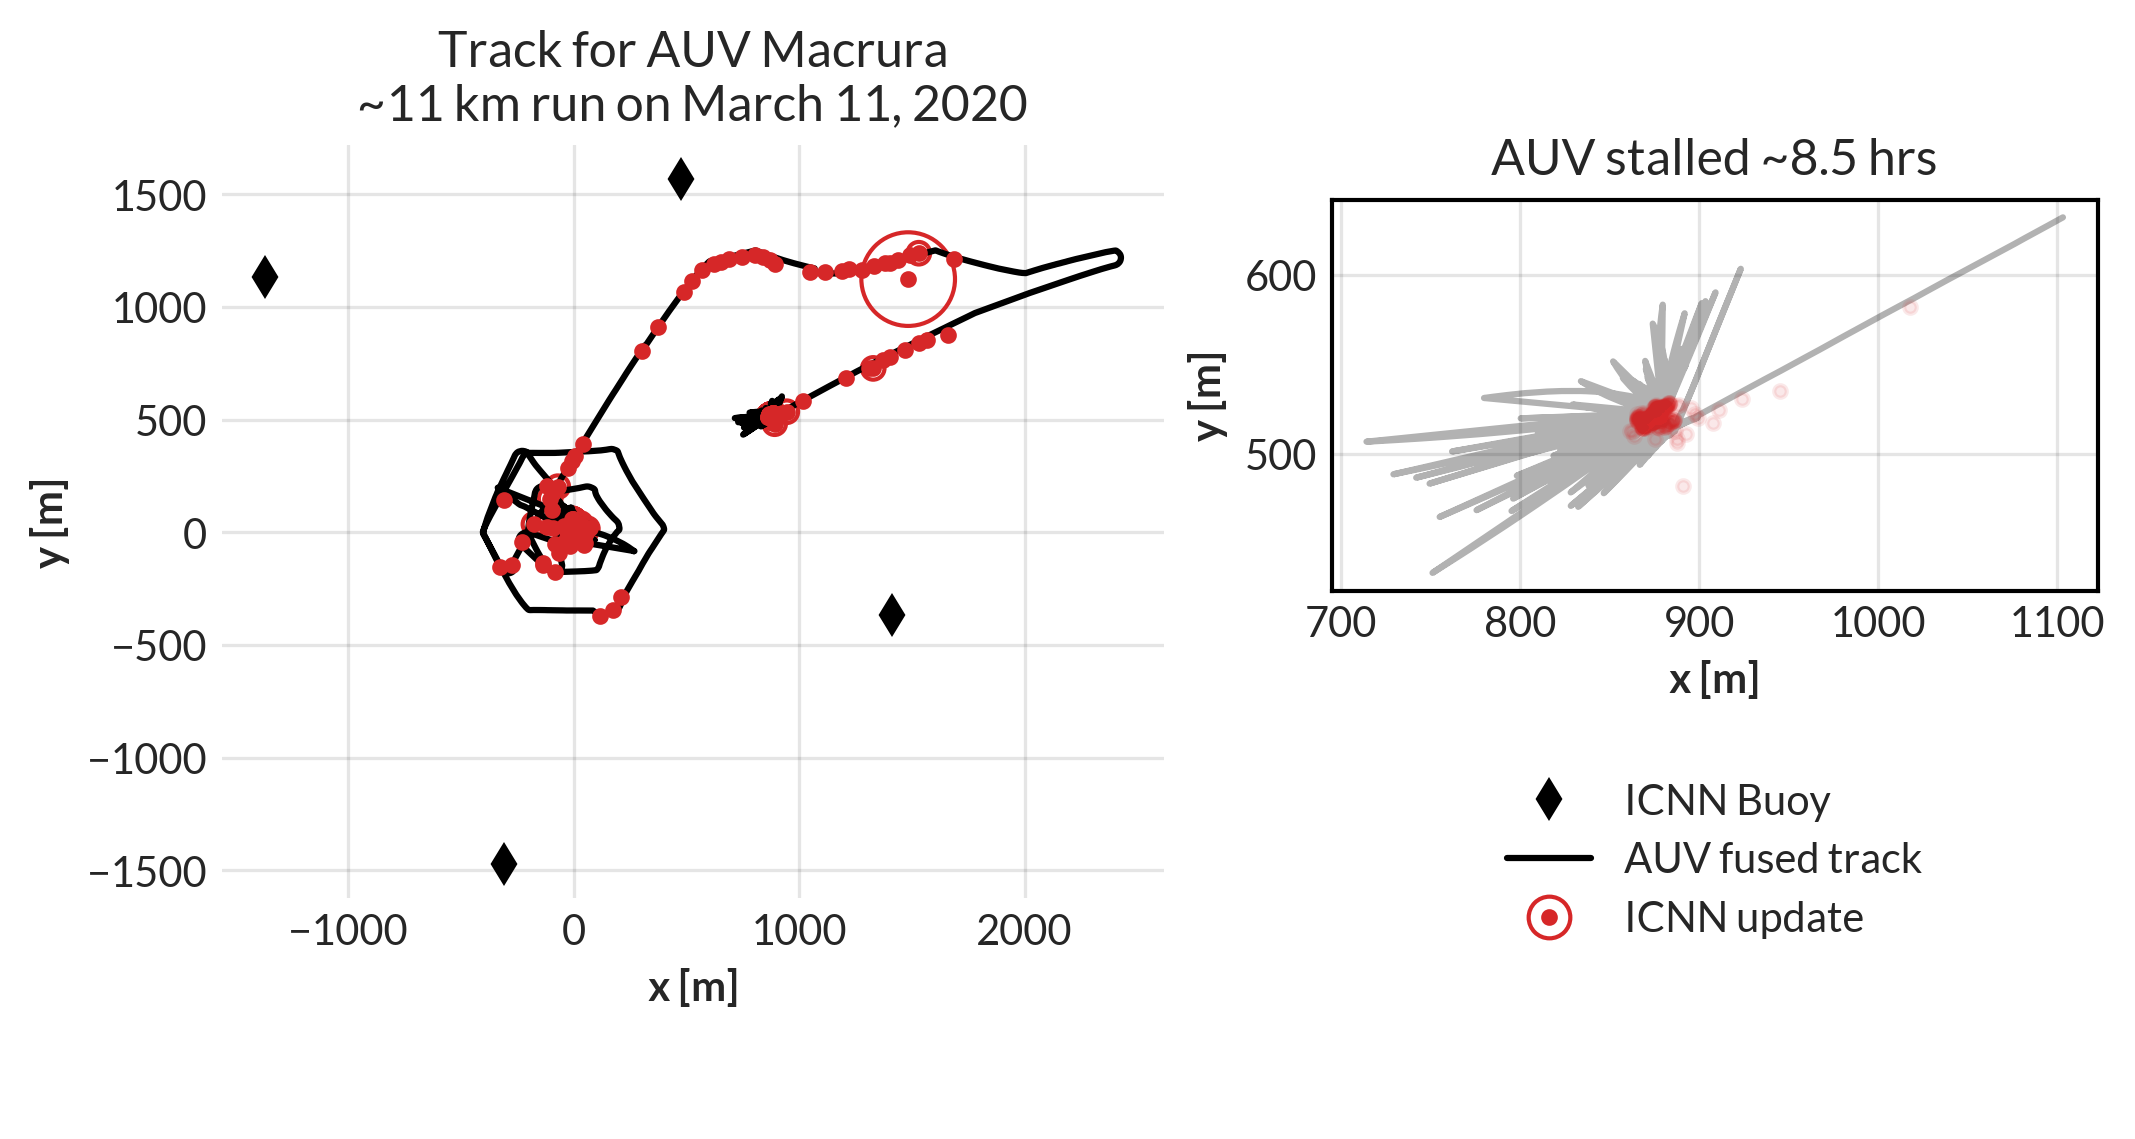
\includegraphics[width=0.7\columnwidth]{figs/auv-track-update.png} \hfill
	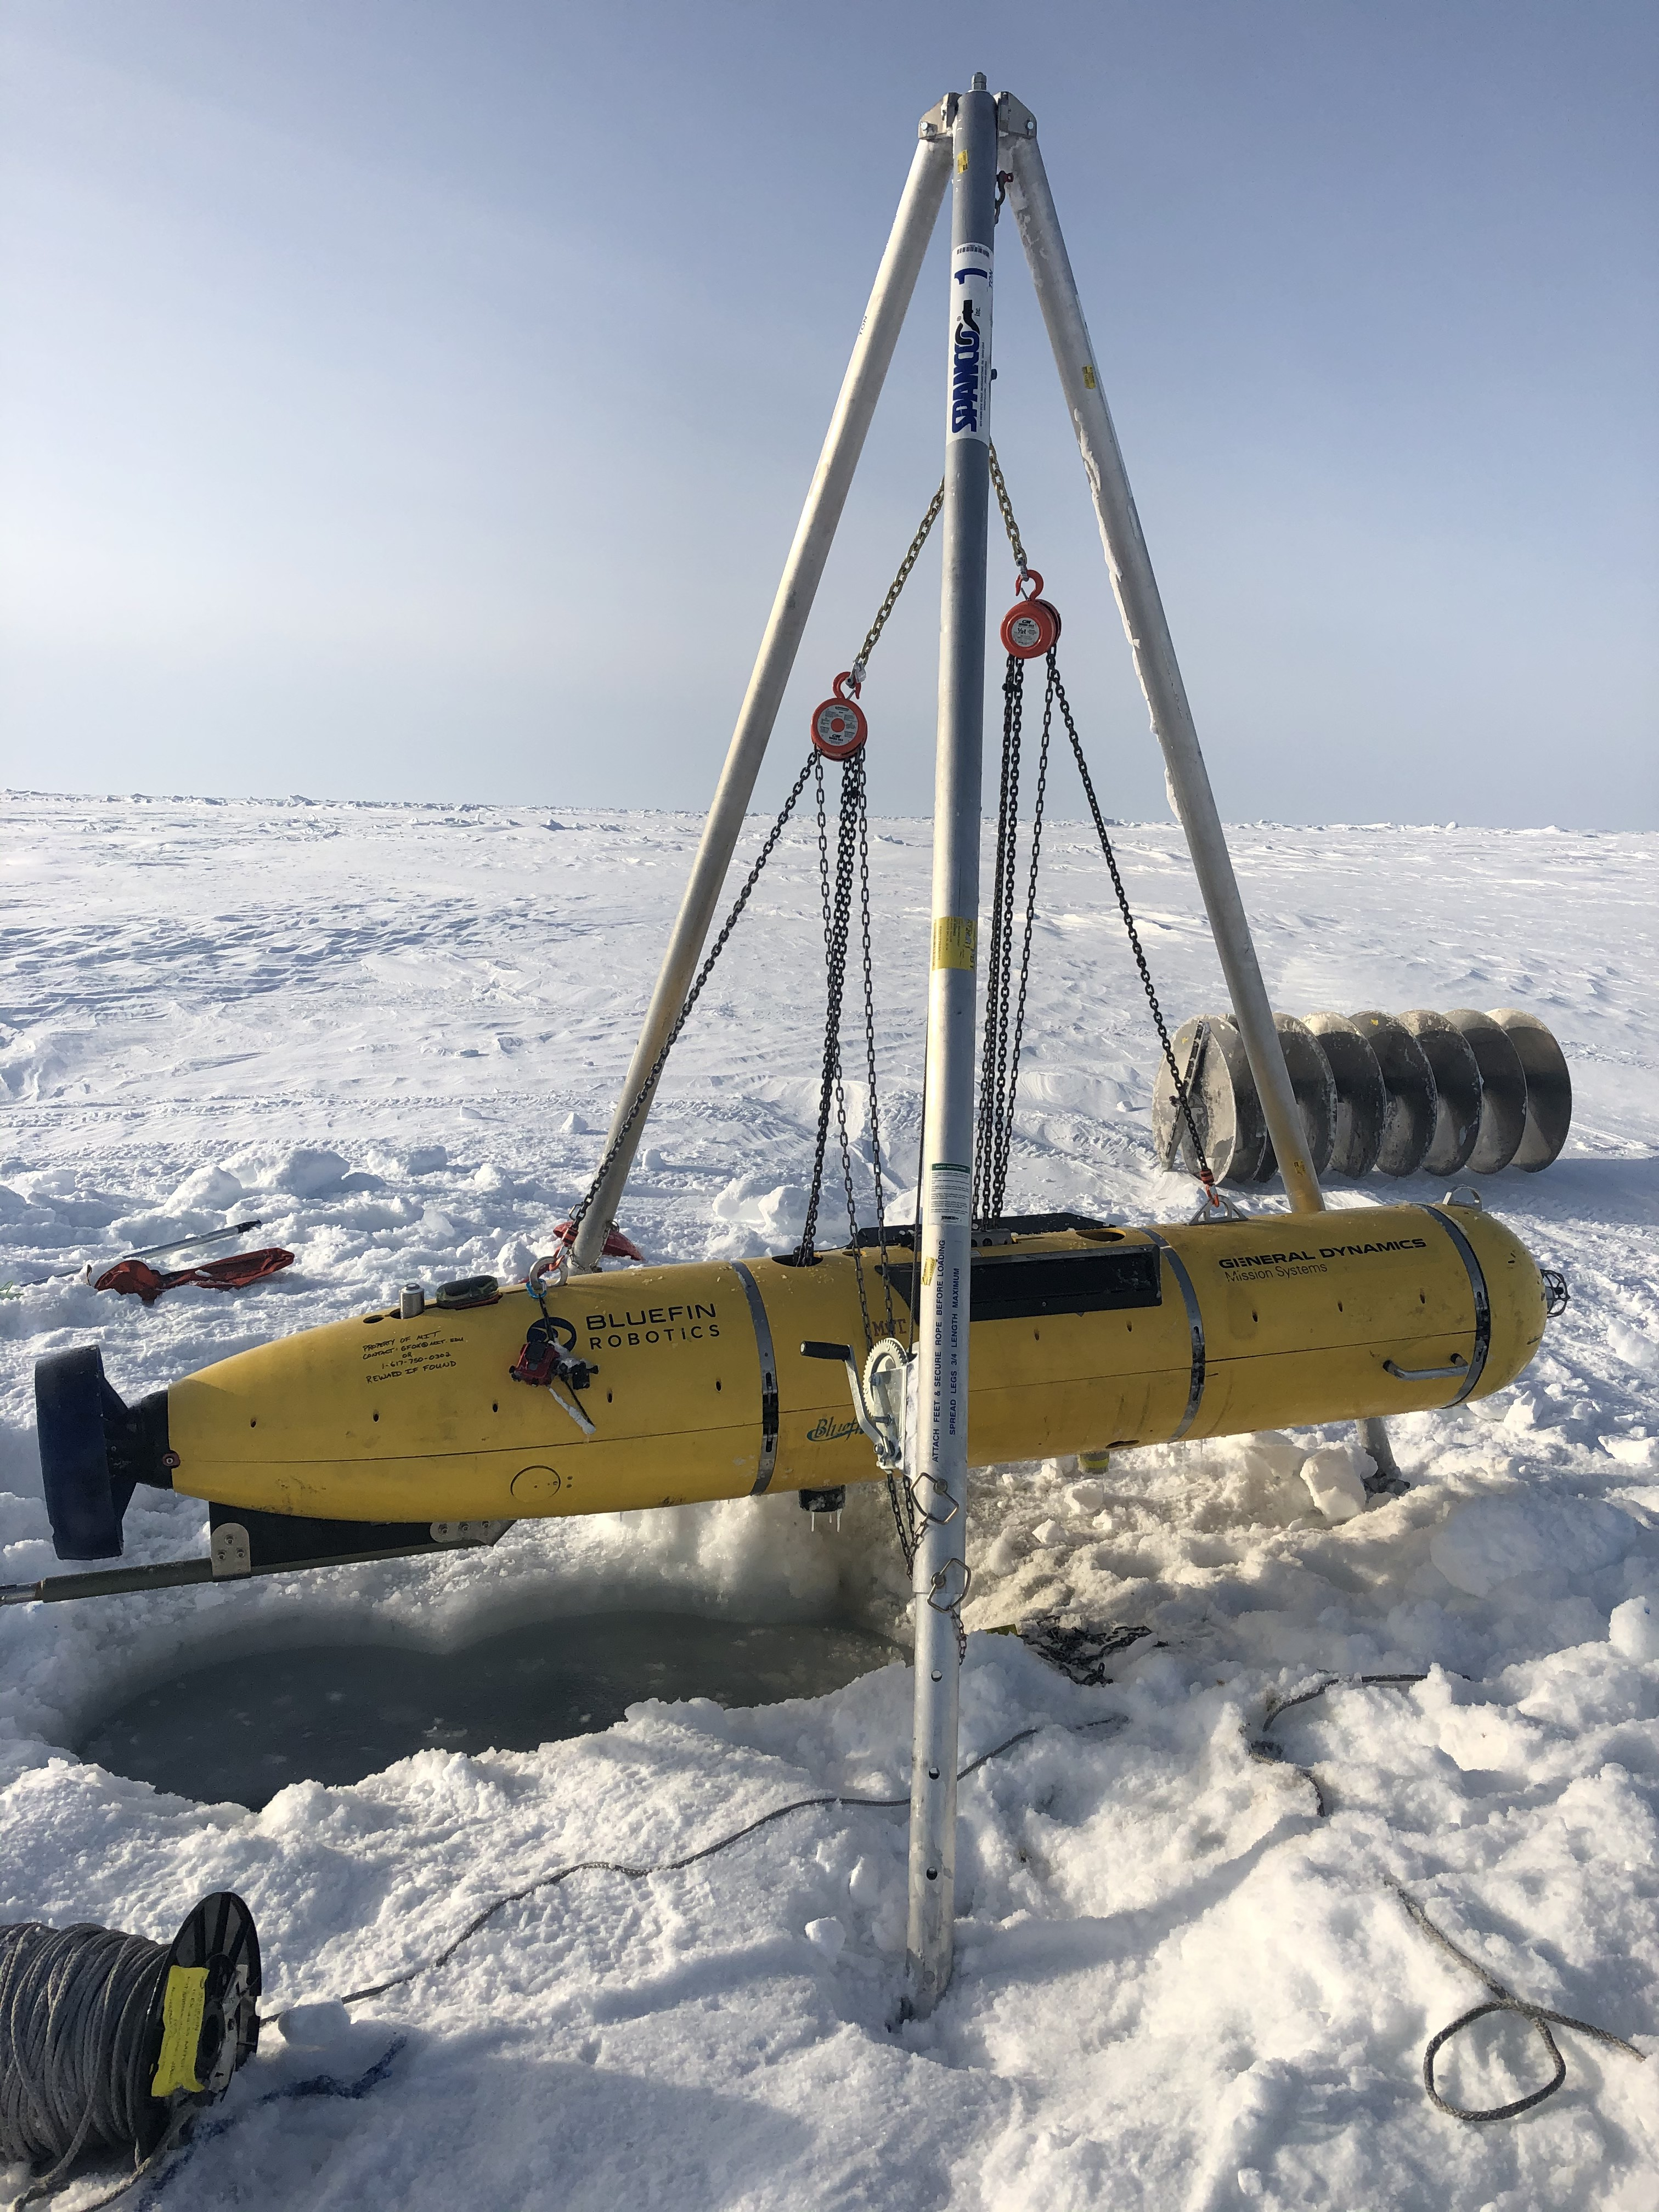
\includegraphics[width=0.28\columnwidth]{figs/Fig1.jpg}
	\caption{The under-ice mission track for AUV Macrura, including the position updates as it stalled underneath the ice overnight. A marker was placed on the ice at the vehicle's estimated self-location. It was recovered after a three day storm within a meter of the marker.}
	\label{fig:vehicleRecovery}
\end{figure}
% include story later on and cite this figure?

\begin{figure}[h!]
	\centering
	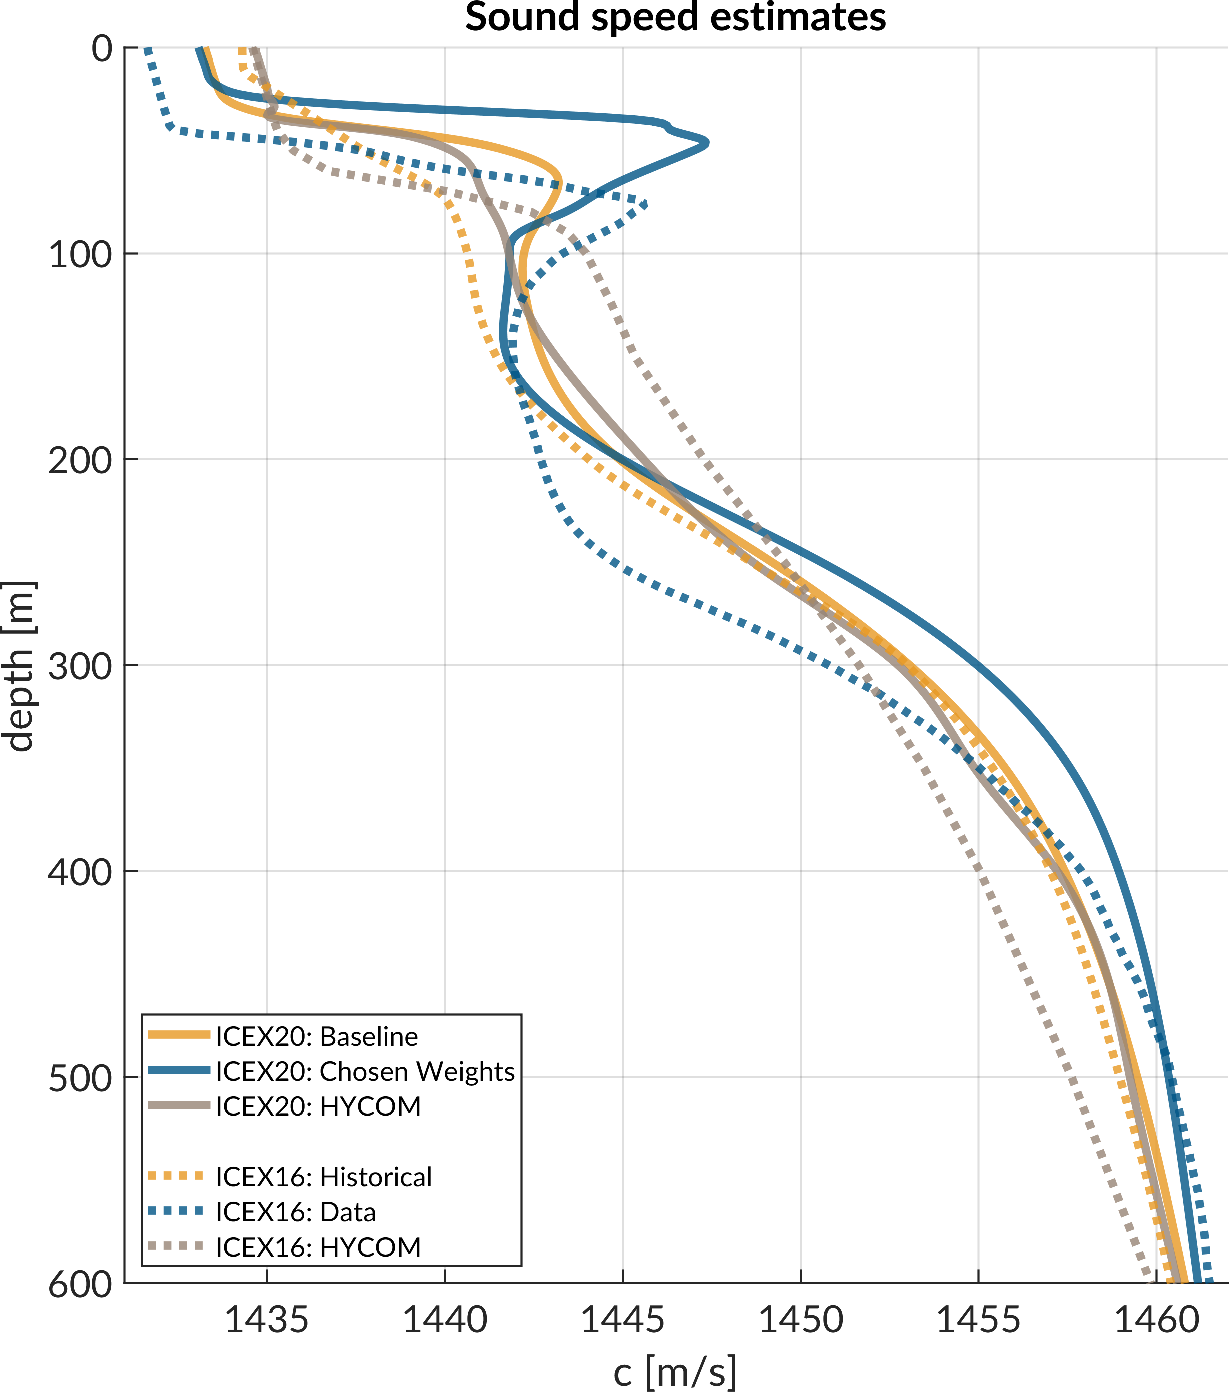
\includegraphics[width=\reprintcolumnwidth]{figs/ssp-gvel-icex20-icex16.pdf}
	\caption{Anticipated sound speed conditions: finish this using stuff from ICEX16, HYCOM, ITP}
	\label{fig:sspExpectation}
\end{figure}

\begin{figure}[h!]
	\centering
	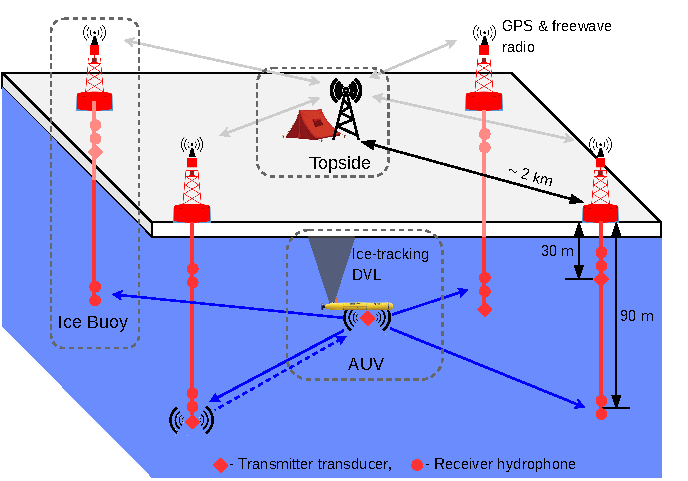
\includegraphics[width=\textwidth]{figs/Fig2.pdf}
	\caption{A schematic overview of the Integrated Communication and Navigation Network (ICNN), which provides joint data-transfer and tracking between AUV and a human decision maker at Topside.}
	\label{fig:icnnOverview}
\end{figure}

\begin{figure}[h!]
  \centering
  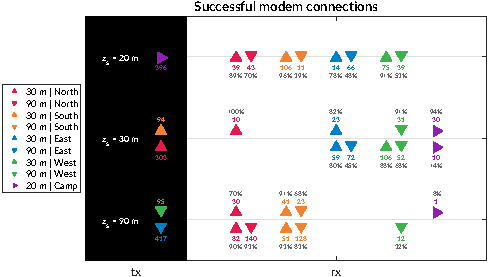
\includegraphics[width=\textwidth]{figs/modem-chart.pdf}
  \caption{An overview of the modem experiment by source and receiver depth and position. The black column on the left, $tx$, shows the source depth, $z_s$. The column on the right, $rx$, shows the receivers with the amount of good contacts. The orientation of the triangles\textemdash sideways, upwards, and downwards\textemdash corresponds to depths of 20, 30, and 90 m.}
  \label{fig:overview}
  \end{figure}

\clearpage
\section{\label{sec:realtime} Real-time pseudorange analysis}

\subsection{Minimal bounce criteria (MBC)}

\subsection{Pseudorange error metrics}

\subsection{Inherent overestimation from the minimal bounce criteria}

\subsubsection{Source depth of 20 m}
\begin{figure}[h!]
  \centering
  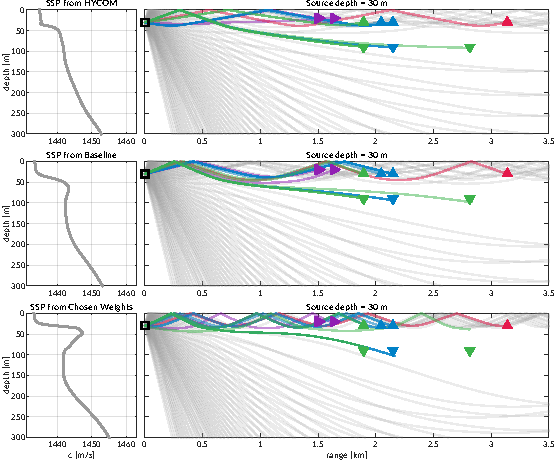
\includegraphics[width=\reprintcolumnwidth]{figs/Fig4.pdf}
  \caption{Eigenrays for beacon to beacon events for each sound speed with a nominal source depth of 20 m. The beacons are highlighted in color/marker coding in Fig. \ref{fig:overview}. The eigenrays are curated from BELLHOP by travel time proximity and are traced in the representative receiver colors over a total ray fan in gray.}
  \label{fig:raytrace-zs20}
\end{figure}


\subsubsection{Source depth of 30 m}
\begin{figure}[h!]
  \centering
  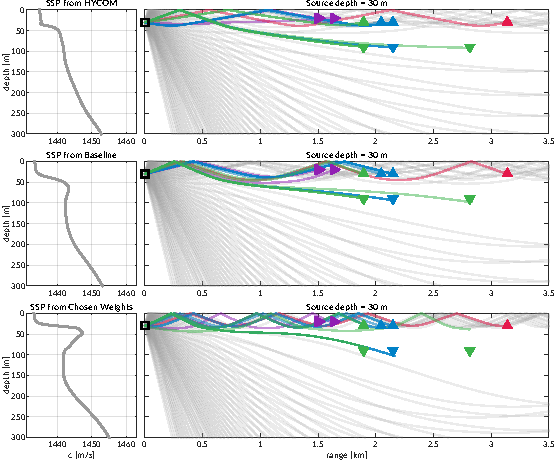
\includegraphics[width=\reprintcolumnwidth]{figs/Fig4.pdf}
  \caption{Eigenrays for beacon to beacon events for each sound speed with a nominal source depth of 30 m. The beacons are highlighted in color/marker coding in Fig. \ref{fig:overview}. The eigenrays are curated from BELLHOP by travel time proximity and are traced in the representative receiver colors over a total ray fan in gray.}
  \label{fig:raytrace-zs30}
\end{figure}

\subsubsection{Source depth of 90 m}
\begin{figure}[h!]
  \centering
  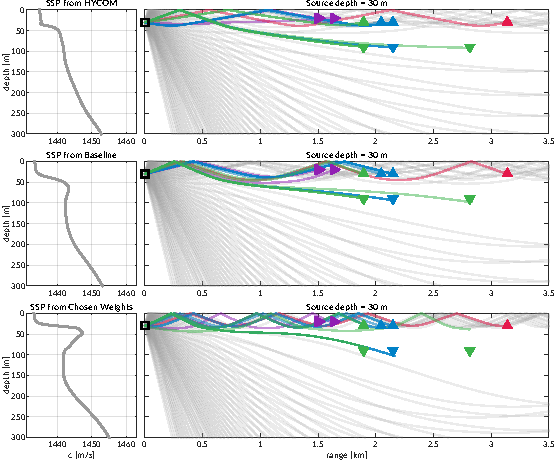
\includegraphics[width=\reprintcolumnwidth]{figs/Fig4.pdf}
  \caption{Eigenrays for beacon to beacon events for each sound speed with a nominal source depth of 90 m. The beacons are highlighted in color/marker coding in Fig. \ref{fig:overview}. The eigenrays are curated from BELLHOP by travel time proximity and are traced in the representative receiver colors over a total ray fan in gray.}
  \label{fig:raytrace-zs90}
\end{figure}

\clearpage
\section{\label{sec:post} Post-processed pseudorange analysis}

\subsection{Nearest bounce criteria (NBC)}

\subsection{Effective sound speed predictions}

\begin{figure}[h!]
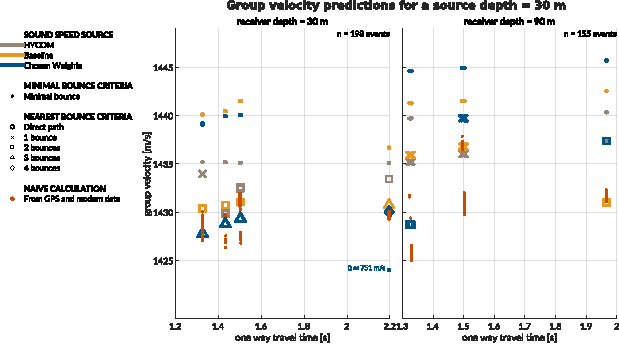
\includegraphics[width=\columnwidth]{figs/Fig5.pdf}
\caption{A comparison of group velocity predictions for all beacon to beacon events in post-processing with a source depth of 30 m, with group velocity on the y-axis and recorded travel time on the x-axis. The left panel is for a receiver depth of 30 m; the right panel for 90 m. The sound speed source is indicated by color. The minimal and nearest bounce criterion are distinguished by different marker shapes, compared to the separately colored red dots showing the naive, data-driven group velocity calculation.}
\label{fig:gvel30}
\end{figure}

\subsection{Pseudorange error metrics}

\begin{figure}[!ht]
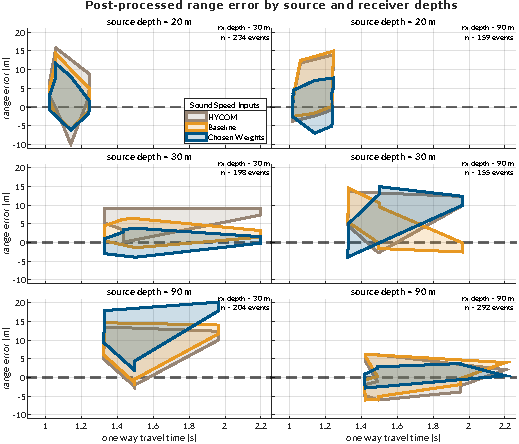
\includegraphics[width=\textwidth]{figs/Fig6.pdf}
\caption{The post-processed range error for source depths of 20, 30, and 90 m, and receiver depths of 30 and 90 m. The dashed gray line shows no error. The shaded region connects the range performance across all events.}
\label{fig:rangeError}
\end{figure}

\clearpage
\section{Trilateration for ICEX20 field data}\label{sec:trilat}

\subsection{Re-positioning beacon to beacon events}

\begin{figure}[!ht]
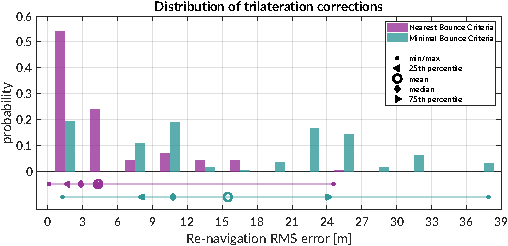
\includegraphics[width=\textwidth]{figs/trilat-stat.pdf}
\caption{WRITE THIS.}
\label{fig:trilat}
\end{figure}

\subsection{Re-navigating AUV Macrura}

FIG A -- error for MBC/NBC (Oscar Fig 6.17). Think about whether to include separate in situ column. Explain why this section uses error whereas previous section uses correction.

I think if we go down this route, we can take out the GNSS noise section entirely. The POMA paper would go over GNSS noise at high latitudes, crossmap, and look at individual drifts. I do not think the crossmap needs to stay in this publication; given small numerical value of the re-positioning trilateration, I think the same point is made (in a better way, actually).

\subsection{Investigating potential GNSS noise}

\begin{figure}[h!]
	\centering
	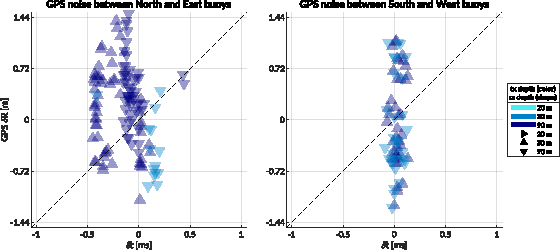
\includegraphics[width=\reprintcolumnwidth]{figs/gps-drift-example.pdf} 
	\caption{A comparison of GPS drift (y-axis) versus OWTT drift (x-axis), colored by source and receiver depth. The physical link between North and East are shown on the top; South and West is on the bottom.}
	\label{fig:gps-drift-example}
\end{figure}

% ================================================== %
% \begin{figure}[ht]
% \includegraphics[width=\reprintcolumnwidth]{figsamp.jpg}
% \caption{\label{fig:FIG1}{Caption here.}}

% \raggedright
% {\color{red}
% Note: The only figure formats allowed are the following:
% .pdf, .ps, .eps, or .jpg. Figure files must be named in this fashion:
% Figure\#.xxx, where ``\#'' is the figure number and ``xxx'' is the file format
% (Figure1.eps, Figure2.jpg, Figure3a.ps, Figure3b.ps, etc).
% }

% [For these sample pages we have used only figsamp.jpg for convenience]
% \end{figure}
% ================================================== %
\FloatBarrier
\clearpage
\begin{acknowledgments}
We acknowledge the significant operational effort spearheaded by the LAMSS ICEX20 team and all our collaborators.
Bhatt was funded by a National Defense, Science, and Engineering Graduate Fellowship.
This work was supported by the Office of Naval Research 322-OA under ICEX20 (N00014-17-1-2474) and Task Force Ocean (N00014-19-1-2716).

\end{acknowledgments}

\bibliography{sampbib}
